The lecture aims to answer the following question: "What is the total angular momentum (or spin) of a bi-partite system if we know the spin of each constituent system?" 

More precisely, in the context of quantum mechanics, consider a spin-$j_A$ system with Hilbert space $\cH_A$ and angular momentum operators $A_1,A_2,A_3$ and a spin-$j_B$ system with Hilbert space $\cH_B$ and angular momentum operators $B_1,B_2,B_3$. Then what is the spin of the composite system with Hilbert space $\cH_A\otimes\cH_B$ and how do we construct the angular momentum operators for this composite system? 

\bp 
\label{prp:AiCommutator}
The operators $A_i\otimes\id_{\cH_B}$ for $i=1,2,3$, satisfy the spin commutation relations. Similarly for $\id_{\cH_A}\otimes B_i$. 
\ep 

\bq 
We shall use the general expression involving the Levi-Civita symbol. Consider the action on a general element $\alpha\otimes\beta\in\cH_A\otimes\cH_B$,
\bi{rCl}
[A_i\otimes \id_{\cH_B}, A_j\otimes \id_{\cH_B}](\alpha\otimes\beta) & := & (A_i\otimes\id_{\cH_B})\big((A_j\alpha) \otimes \beta\big) - (A_j\otimes\id_{\cH_B})\big((A_i\alpha) \otimes \beta\big) \\
& = & A_i(A_j\alpha) \otimes\beta - A_j(A_i\alpha)\otimes\beta \\
& = & \big((A_iA_j-A_jA_i)\alpha\big)\otimes\beta \\
& = & \big([A_i,A_j]\alpha \big)\otimes \beta \\
& = & i\epsilon_{ijk} (A_k\alpha)\otimes\beta \\
& = & i\epsilon_{ijk} (A_k\otimes\id_{\cH_B})(\alpha\otimes\beta),
\ei 
which because $\alpha\otimes\beta$ was arbitary (or equivalently by the linearity of the operators) this holds for \emph{any} element of $\cH_A\otimes\cH_B$.

The method is identical for the $\id_{\cH_A}\otimes B_i$ case. 
\eq 

Now before moving on recall (page 137) that we have an ON-eigenbasis\footnote{ON here stands for orthonormal.} for each constituent system. That is if $A^2$ is the Casimir operator for the spin-$j_A$ system then we have the ON-eigenbasis 
\bse 
\{\alpha_{j_A}^{m_A}\}_{m_A=-j_A,...,j_A}
\ese 
with 
\bse
A^2\alpha_{j_A}^{m_A} = j_A(j_A+1)\alpha_{j_A}^{m_A}.
\ese 
Similarly we have $B^2$ and $\{\beta_{j_B}^{m_B}\}$, $m_B=-j_B,...,j_B$.

\subsection{Total Spin}

\br 
From now on we shall simply write $\b1$ instead of $\id_{\cH_A}$ and $\id_{\cH_B}$, and the placement relative to the tensor product will indicate which is meant. 
\er 

In everything that follows it is important to note that $j_A$ and $j_B$ are fixed. This condition shall come in use later.  

\bd 
We define the self adjoint angular momentum operators $J_1,J_2,J_3$ on the composite space $\cH_A\otimes\cH_B$ as 
\bse 
J_i := A_i\otimes \b1 + \b1 \otimes B_i,
\ese 
and we call them the \emph{total spin operators}.
\ed 

\bq (that they obey the spin commutation relations)

Consider
\bi{rCl}
[A_i\otimes\b1,\b1\otimes B_j](\alpha\otimes\beta) & := & (A_i\otimes\b1)(\alpha\otimes B_j\beta) - (\b1\otimes B_j)(A_i\alpha \otimes \beta) \\
& = & (A_i\alpha)\otimes(B_j\beta) - (A_i\alpha)\otimes(B_j\beta) \\
& = & 0,
\ei 
which from the fact that the commutator bracket is antisymmetric in its entries, along with \Cref{prp:AiCommutator} gives the result. 
\eq 

\bd 
We define the Casimir operator for the composite system as always, 
\bse 
J^2 := \sum_{i=1}^3 J_i\circ J_i.
\ese 
\ed 

\bd 
We define the \emph{total ladder operators} as 
\bse
J_{\pm} := A_{\pm}\otimes\b1 + \b1\otimes B_{\pm}.
\ese 
\ed 

We now want to find the common eigenvalues of $J^2$ and one of the total spin operators, $J_3$ say. We will show the following results:
\bi{rCl}
\sigma(J^2) & = & \{|j_A-j_B|,...,j_A+j_B\} \\
\sigma(J_3) & = & \{-(j_A+j_B),...,j_A+j_B\}.
\ei 

\br 
Note from \Cref{thrm:SigmaTensorProduct}, we can already obtain the second of these two results. That is 
\bi{rCl}
\sigma(J_3) & := & \sigma(A_3\otimes\b1 + \b1\otimes B_3) \\
& = & \overline{\sigma(A_3) + \sigma(B_3)} \\
& = & \overline{\{-j_A,...,j_A\} + \{-j_B,...,j_B\}} \\
& = & \{-(j_A+j_B),...,j_A+j_B\}.
\ei
\er 

\subsection{Eigenbasis For The Composite System in Terms of Simultaneous Eigenvectors of $A^2\otimes\b1$, $\b1\otimes B^2$, $A_3\otimes\b1$ and $\b1\otimes B^3$}

We already know that $\{\alpha_{j_A}^{m_A}\otimes\beta_{j_B}^{m_B}\}$ for $m_A=-j_A,...,j_A$ and $m_B=-j_B,...,j_B$, are common eigenvectors of all four operators with eigenvalues 
\bi{rCl}
(A^2\otimes\b1)(\alpha_{j_A}^{m_A}\otimes\beta_{j_B}^{m_B}) & = & j_A(j_A+1)\alpha_{j_A}^{m_A}\otimes\beta_{j_B}^{m_B} \\
(\b1\otimes B^2)(\alpha_{j_A}^{m_A}\otimes\beta_{j_B}^{m_B}) & = & j_B(j_B+1)\alpha_{j_A}^{m_A}\otimes\beta_{j_B}^{m_B} \\
(A_3\otimes\b1)(\alpha_{j_A}^{m_A}\otimes\beta_{j_B}^{m_B}) & = & m_A\alpha_{j_A}^{m_A}\otimes\beta_{j_B}^{m_B} \\
(\b1\otimes B_3)(\alpha_{j_A}^{m_A}\otimes\beta_{j_B}^{m_B}) & = & m_B\alpha_{j_A}^{m_A}\otimes\beta_{j_B}^{m_B}.
\ei 
It also follows from the definition of the composite inner product that it is an ON-eigenbasis. That is, 
\bi{rCl} 
\braket{\alpha_{j_A}^{m_A}\otimes\beta_{j_B}^{m_B}}{ \alpha_{j'_A}^{m'_A}\otimes\beta_{j'_B}^{m'_B}}_{12} & := & \braket{\alpha_{j_A}^{m_A}}{\alpha_{j'_A}^{m'_A}}_1 \braket{\alpha_{j_B}^{m_B}}{\alpha_{j'_B}^{m'_B}}_2 \\
& = & \delta_{j_A,j'_A}\delta_{m_A,m'_A}\delta_{j_B,j'_B}\delta_{m_B,m'_B}.
\ei

So we have an ON-eigenbasis for the eigenvectors of these operators. As we shall see, this basis shall be crucial to finding the eigenvectors of $J^2$ and $J_3$, and so their spectra. 

\subsection{Conversion to Eigenbasis in Terms of $J^2$, $J_3$, $A^2\otimes\b1$, $\b1\otimes B^2$}

The first thing we note here is that not only is $J^2$ a Casimir operator of $J_1,J_2,J_3$ but so are $A^2\otimes\b1$ and $\b1\otimes B^2$. This is seen straight from the linearity of the commutator bracket, 
\bi{rCl}
[A^2\otimes\b1,J_i] & := & [A^2\otimes\b1,A_i\otimes\b1+\b1\otimes B_i] \\
& = & [A^2\otimes\b1,A_i\otimes\b1] + [A^2\otimes\b1,\b1\otimes B_i] \\
& = & 0,
\ei 
as each bracket vanishes. Similarly for $\b1\otimes B^2$. We also have, using $\Cref{cor:ABCCommutator}$ that 
\bse
[J^2,A^2\otimes\b1] = 0 = [J^2,\b1\otimes B^2].
\ese 

We can therefore consider eigenvectors of $J_3$ that are not only common to $J^2$ but also to $A^2\otimes\b1$ and $\b1\otimes B^2$, and so we have a simultaneous eigenbasis, $\{\xi_{j,j_A,j_B}^m\}$ which satisfies 
\bi{rCl}
J^2 \xi_{j,j_A,j_B}^m & = & j(j+1)\xi_{j,j_A,j_B}^m \\
J_3 \xi_{j,j_A,j_B}^m & = & m \xi_{j,j_A,j_B}^m \\
(A^2\otimes\b1)\xi_{j,j_A,j_B}^m & = & j_A(j_A+1) \xi_{j,j_A,j_B}^m \\
(\b1\otimes B^2)\xi_{j,j_A,j_B}^m & = & j_B(j_B+1)\xi_{j,j_A,j_B}^m.
\ei 

Now since we already have the ON-eigenbasis $\{\alpha_{j_A}^{m_A}\otimes\beta_{j_B}^{m_B}\}$ for $A^2\otimes\b1$ and $\b1\otimes B^2$ it follows (by the definition of a basis) that this new basis can be expanded as\footnote{We shall drop the subscript on the inner product here to lighten notation, but obviously it is the one for the composite Hilbert space.} 
\bse 
\xi_{j,j_A,j_B}^m = \sum_{m_A=-j_A}^{j_A}\sum_{m_B=-j_B}^{j_B}\braket{\alpha_{j_A}^{m_A}\otimes\beta_{j_B}^{m_B}}{\xi_{j,j_A,j_B}} \alpha_{j_A}^{m_A}\otimes\beta_{j_B}^{m_B}.  
\ese 

\bd 
We define the \emph{Clebsch-Gordan coefficients} (CGc) as 
\bse 
C_{j,j_A,j_B}^{m,m_A,m_B} := \braket{\alpha_{j_A}^{m_A}\otimes\beta_{j_B}^{m_B}}{\xi_{j,j_A,j_B}},
\ese 
and so we can rewrite the previous expression as 
\bse 
\xi_{j,j_A,j_B}^m = \sum_{m_A=-j_A}^{j_A}\sum_{m_B=-j_B}^{j_B} C_{j,j_A,j_B}^{m,m_A,m_B} \alpha_{j_A}^{m_A}\otimes\beta_{j_B}^{m_B}.  
\ese 
\ed 

\br 
The Clebsch-Gordan coefficients are just complex numbers. Although they might be rather difficult to calculate in practice, the method should now be clear. All we need to do is calculate the CGc and then we instantly have our new eigenbasis, and so we get the spectra for $J^2$ and $J_3$. 
\er 

As just noted, they are pretty hard to calculate, stemming from the fact that $\xi_{j,j_A,j_B}^m$ appears both on the LHS and within the inner product, however we can do it indirectly. This forms the remainder of this lecture. 

The strategy is as follows: start from some convenient eigenvector $\xi_{j,j_A,j_B}^j$ and its associated CGcs, then use the ladder operators to obtain the eigenvector $\xi_{j,j_A,j_B}^{j\pm1}$ and the resulting CGcs. We will then change the value of $j$ itself and repeat the process. In this manner we will build up a table of CGcs.

\begin{center}
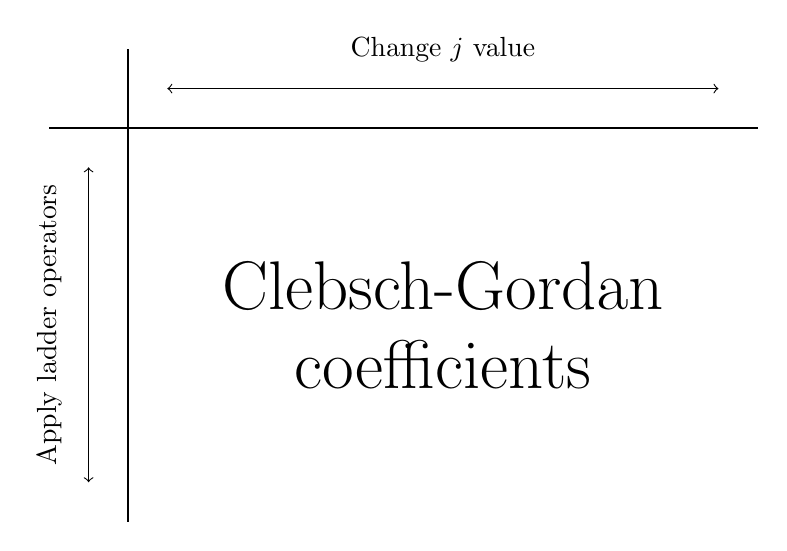
\begin{tikzpicture}
\draw[thick] (-1,0) -- (8,0);
\draw[thick] (0,1) -- (0,-5);
\draw[<->] (0.5,0.5) -- (7.5,0.5);
\node at (4,1) {Change $j$ value};
\draw[<->] (-0.5,-0.5) -- (-0.5,-4.5);
\node[rotate=90] at (-1,-2.5) {Apply ladder operators};
\node at (4,-2) {\Huge{Clebsch-Gordan}};
\node at (4,-3) {\Huge{coefficients}};
\end{tikzpicture}
\end{center}

\subsection{Value of $m$}

Consider the action of $J_3$ on both bases, 
\bi{rCl}
J_3\xi_{j,j_A,j_B}^m & = & m\xi_{j,j_A,j_B} \\
J_3 (\alpha_{j_A}^{m_a} \otimes \beta_{j_B}^{m_B}) & = & (m_A+m_B)(\alpha_{j_A}^{m_a} \otimes \beta_{j_B}^{m_B}).
\ei 
Then, from the fact that the CGcs are simply complex numbers and the fact that $J_3$ is linear, it follows from the expansion equation that we require 
\bse 
m = m_A + m_B.
\ese 
In other words, whenever $m\neq m_A+m+B$, we require that the CGc vanishes. We can, therefore, place this as a constraint on our summands giving us 
\bse 
\xi_{j,j_A,j_B}^m = \sum_{\substack{m_A,m_B \\ m_A+m_B=m}} C_{j,j_A,j_B}^{m,m_A,m_B} (\alpha_{j_A}^{m_a} \otimes \beta_{j_B}^{m_B}),
\ese 
where we have left the ranges of $m_A/m_B$ out, but they are of course just $-j_A,...,j_A$ and $-j_B,...,j_B$.

\subsection{Clebsch-Gordan Coefficients for Maximal $j$}

We are now in a position to choose our convenient initial eigenvector. It follows from the ranges of $m_A$ and $m_B$ along with the condition $m=m_A+m_B$ and $m=-j,...,j$ that the maximum value $j$ can take is $j_A+j_B$. It follows then that 
\bse 
\xi_{j_A+j_B,j_A,j_B}^{j_A+j_B} = C_{j_A+j_B,j_A,j_B}^{j_A+j_B,j_A,j_B} (\alpha_{j_A}^{j_A}\otimes\beta_{j_B}^{j_B}),
\ese 
and all other CGcs at the level $C_{j_A+j_B,j_A,j_B}^{j_A+j_B, -, -}$ vanish. Then from the fact that both eigenbases are normalised we know that 
\bse 
\big|C_{j_A+j_B,j_A,j_B}^{j_A+j_B,j_A,j_B}\big|^2 = 1,
\ese 
and so the two eigenvectors vary only by a complex phase. However, seeing as we are only interested in eigenvalues here, and an \emph{overall} phase plays no effect on the eigenvalue, we are free to set this phase however we like. We choose it such that 
\bse 
C_{j_A+j_B,j_A,j_B}^{j_A+j_B,j_A,j_B} = 1.
\ese 

We can now start applying the ladder operators to lower the value of $m=j_A+j_B$. Using \Cref{prp:LadderCoefficients} we have 
\bi{rCl}
J_- \xi_{j_A+j_B,j_A,j_B}^{j_A+j_B} & = & \sqrt{(j_A+j_B)(j_A+j_B+1)-(j_A+j_B)(j_A+j_B-1)}\xi_{j_A+j_B,j_A,j_B}^{j_A+j_B-1} \\
& = & \sqrt{2(j_A+j_B)}\xi_{j_A+j_B,j_A,j_B}^{j_A+j_B-1}
\ei 
However we equally have 
\bi{rCl}
J_-(\alpha_{j_A}^{j_A}\otimes\beta_{j_B}^{j_B}) & = & (A_-\otimes\b1 +\b1\otimes B_-) (\alpha_{j_A}^{j_A}\otimes\beta_{j_B}^{j_B}) \\
& = & \sqrt{2j_A}(\alpha_{j_A}^{j_A-1}\otimes\beta_{j_B}^{j_B}) + \sqrt{2j_B}(\alpha_{j_A}^{j_A}\otimes\beta_{j_B}^{j_B-1}).
\ei
Then, equating these two, we obtain 
\bi{rCl}
C_{j_A+j_B,j_A,j_B}^{j_A+j_B-1,j_A-1,j_B} & = & \sqrt{\frac{j_A}{j_A+j_B}} \\
C_{j_A+j_B,j_A,j_B}^{j_A+j_B-1,j_A,j_B-1} & = & \sqrt{\frac{j_B}{j_A+j_B}},
\ei 
with all other CGcs at this level vanishing. 

We can repeat this process to obtain the CGcs at the level $C_{j_A+j_B,j_A,j_B}^{j_A+j_B-2,-,-}$, and iterate until we reach $m=-(j_A+j_B)$, which is where it must terminate. 

\subsection{Clebsch-Gordan Coefficients For Lower Than Max $j$}

We now wish to reduce $j$ itself to produce the second column of our table. We first need to ask what the next highest allowed $j$ value is. Recalling that $j\in\N_0/2$ we might try $j_A+j_B-1/2$, however this is not allowed. The answer to why follows simply from the fact that $j_A$ and $j_B$ themselves are fixed, so all we can change is $m_A$ and $m_B$, which must change in integer steps. Combining this with the $m=m_A+m_B$, which holds generally, we would not be able to get $m=-j,...,j$. That is, the next CGcs are of level $C_{j_A+j_B-1,j_A,j_B}^{j_A+j_B-1,-,-}$. Then using the fact that there are only two ways to obtain this (either $m_A\to m_A-1$ or $m_B\to m_B-1$) we have 
\bse 
\xi_{j_A+j_B-1,j_A,j_B}^{j_A+j_B-1} = C_{j_A+j_B-1,j_A,j_B}^{j_A+j_B-1,j_A-1,j_B}(\alpha_{j_A}^{j_A-1}\otimes\beta_{j_B}^{j_B}) + C_{j_A+j_B-1,j_A,j_B}^{j_A+j_B-1,j_A,j_B-1}(\alpha_{j_A}^{j_A}\otimes\beta_{j_B}^{j_B-1}).
\ese 

We then use the fact that the eigenvectors in this equation are all orthonormal to obtain 
\bse 
1 = \big|C_{j_A+j_B-1,j_A,j_B}^{j_A+j_B-1,j_A-1,j_B}\big|^2 + \big|C_{j_A+j_B-1,j_A,j_B}^{j_A+j_B-1,j_A,j_B-1}\big|^2,
\ese 
and we also use the fact that the RHS eigenvectors are the same here as with the $J_-$ case above however the LHS eigenvectors are necessarily orthogonal to give 
\bi{rCl} 
\overline{C_{j_A+j_B,j_A,j_B}^{j_A+j_B-1,j_A-1,j_B}}\cdot C_{j_A+j_B-1,j_A,j_B}^{j_A+j_B-1,j_A-1,j_B} & = & - \overline{C_{j_A+j_B,j_A,j_B}^{j_A+j_B-1,j_A,j_B-1}}\cdot C_{j_A+j_B-1,j_A,j_B}^{j_A+j_B-1,j_A,j_B-1} \\
\sqrt{\frac{j_A}{j_A+j_B}}\cdot C_{j_A+j_B-1,j_A,j_B}^{j_A+j_B-1,j_A-1,j_B} & = & -\sqrt{\frac{j_B}{j_A+j_B}}\cdot C_{j_A+j_B-1,j_A,j_B}^{j_A+j_B-1,j_A,j_B-1} \\
C_{j_A+j_B-1,j_A,j_B}^{j_A+j_B-1,j_A-1,j_B} & = & -\sqrt{\frac{j_B}{j_A}}\cdot  C_{j_A+j_B-1,j_A,j_B}^{j_A+j_B-1,j_A,j_B-1}.
\ei 

Solving simultaneously, 
\bi{rCl}
\bigg(\frac{j_B}{j_A} +1\bigg)\big|C_{j_A+j_B-1,j_A,j_B}^{j_A+j_B-1,j_A,j_B-1}\big|^2 & = & 1 \\
\big|C_{j_A+j_B-1,j_A,j_B}^{j_A+j_B-1,j_A,j_B-1}\big| & = & \sqrt{\frac{j_A}{j_A+j_B}} \\
\implies \big|C_{j_A+j_B-1,j_A,j_B}^{j_A+j_B-1,j_A-1,j_B}\big| & = & -\sqrt{\frac{j_B}{j_A+j_B}}
\ei 
Finally we just fix the phases as we want to give 
\bse
C_{j_A+j_B-1,j_A,j_B}^{j_A+j_B-1,j_A,j_B-1} = \sqrt{\frac{j_A}{j_A+j_B}}, \qquad \qquad  C_{j_A+j_B-1,j_A,j_B}^{j_A+j_B-1,j_A-1,j_B} = -\sqrt{\frac{j_B}{j_A+j_B}}.
\ese

We can then apply the $J_-$ operator as before to move down this column. We can repeat this process of lowering $j$ again to obtain the third column, and iterate until we reach $j=|j_A-j_B|$, where it must terminate. We see that this is the termination point quickly from $m=-j,...,j$ along with $m=m_A+m_B$. On the next page I have included a table (from David J. Griffiths' QM book) for some calculated CGcs. As we can see... they're not pretty things.

\subsection{Total Spin of Composite System}

We conclude, then, that in quantum mechanics when we want to compose a spin-$j_A$ system with a spin-$j_B$ system we do \emph{not} just get a spin-$j_A+j_B$ system, but instead we get the direct sum 
\bse
(\text{spin-}_{j_A+j_B}) \oplus (\text{spin-}_{j_A+j_B-1}) \oplus ... \oplus (\text{spin-}_{|j_A-j_B|}).
\ese 

\begin{center}
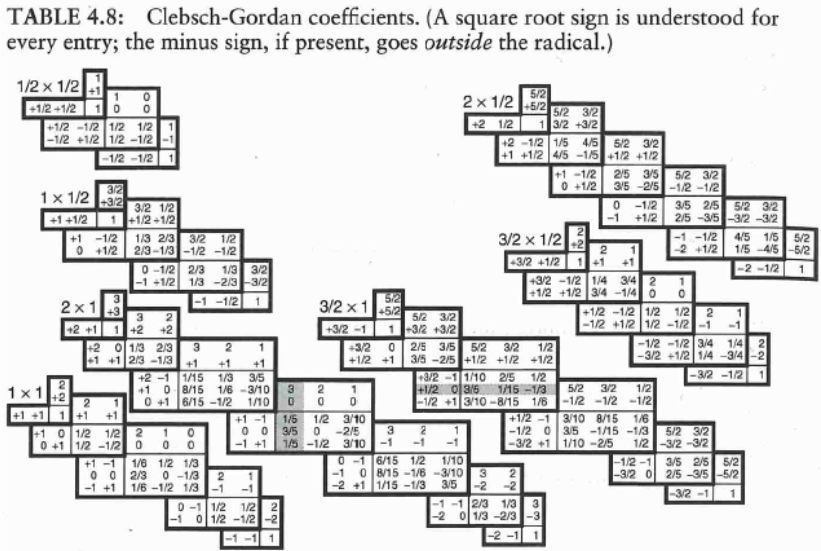
\includegraphics[scale=0.7,angle=90, origin=c]{graphics/ClebschGordan.png}
\end{center}